% This is a Basic Assignment Paper but with code, URLs, and hyperlinks included.

\documentclass[openany]{report}

% Preamble

\usepackage[margin=1in]{geometry}
\usepackage{amsfonts, amsmath, amssymb}
\usepackage{fancyhdr, float, graphicx}
\usepackage[utf8]{inputenc} % For international characters
\usepackage[T1]{fontenc}    % Output font encoding
\usepackage{fouriernc}      % New Century Schoolbook font
\usepackage[nottoc, notlot, notlof]{tocbibind}
\usepackage{listings}
\usepackage{xcolor}
\usepackage{hyperref}

\hypersetup{
    colorlinks=true,
    linkcolor=black,
    filecolor=magenta,
    urlcolor=blue,
    pdfpagemode=FullScreen,
}

\definecolor{codegreen}{rgb}{0,0.6,0}
\definecolor{codegray}{rgb}{0.5,0.5,0.5}
\definecolor{codepurple}{rgb}{0.58,0,0.82}
\definecolor{backcolour}{rgb}{0.95,0.95,0.92}

\lstdefinestyle{mystyle}{
    backgroundcolor=\color{backcolour},
    commentstyle=\color{codegreen},
    keywordstyle=\color{magenta},
    numberstyle=\tiny\color{codegray},
    stringstyle=\color{codepurple},
    basicstyle=\ttfamily\footnotesize,
    breaklines=true,
    captionpos=b,
    numbers=left,
    numbersep=5pt,
    tabsize=2,
    showspaces=false,
    showstringspaces=false,
    showtabs=false
}

\lstset{style=mystyle}

% Header and Footer
\pagestyle{fancy}
\fancyhead{}
\fancyfoot{}
\fancyhead[L]{\textit{\Large{Report - 4th Year B. Tech}}}
\fancyhead[R]{\textit{Krishnaraj Thadesar}}
\fancyfoot[C]{\thepage}
\renewcommand{\footrulewidth}{1pt}

\begin{document}


%========================================
\chapter{Individual Contribution}

\begin{figure}[H]
    \centering
    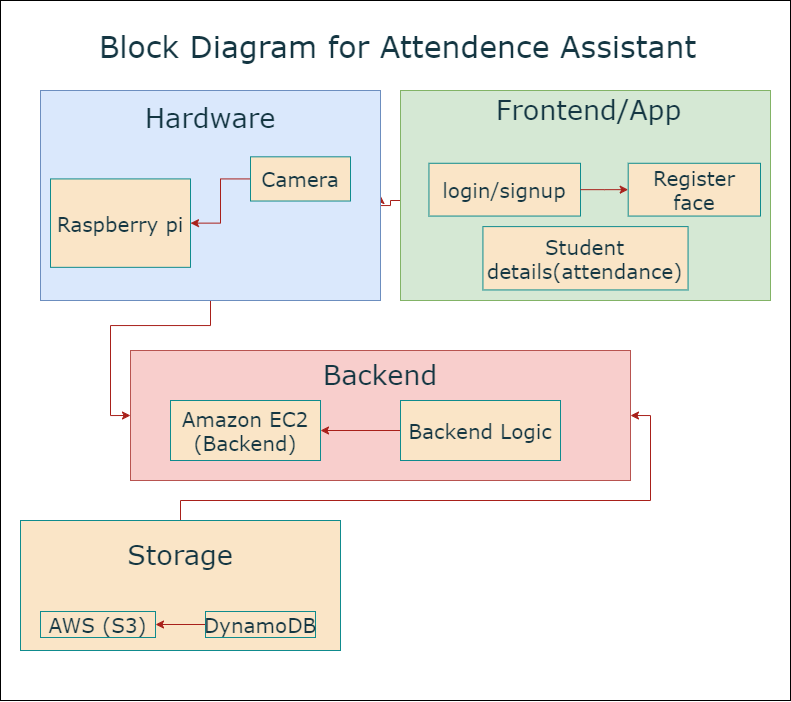
\includegraphics[width=0.95\textwidth]{../imgs/block diagram.png}
    \caption{Block Diagram highlighting the modules supported by Parth Zarekar.}
    \label{fig:block_diagram_parth}
  \end{figure}
%========================================
\section{Problem Statement}
Design and implement the backend API and face‐recognition engine for the Attendance‐Assistant system.

\section{Student Details}
\textbf{Krishnaraj Thadesar} \\
\textbf{PRN:} 1032210888 \\
\textbf{Roll Number:} 15 \\
\textbf{Panel:} A \\

\section{Module Title}
Backend \& Face‐Recognition Engine

\section{Project’s Module Scope (Individual Perspective)}
End‐to‐end implementation of all backend services, face‐encoding storage and lookup, handling concurrent API calls from clients, all hosted locally via Docker.
\begin{figure}[H]
    \centering
    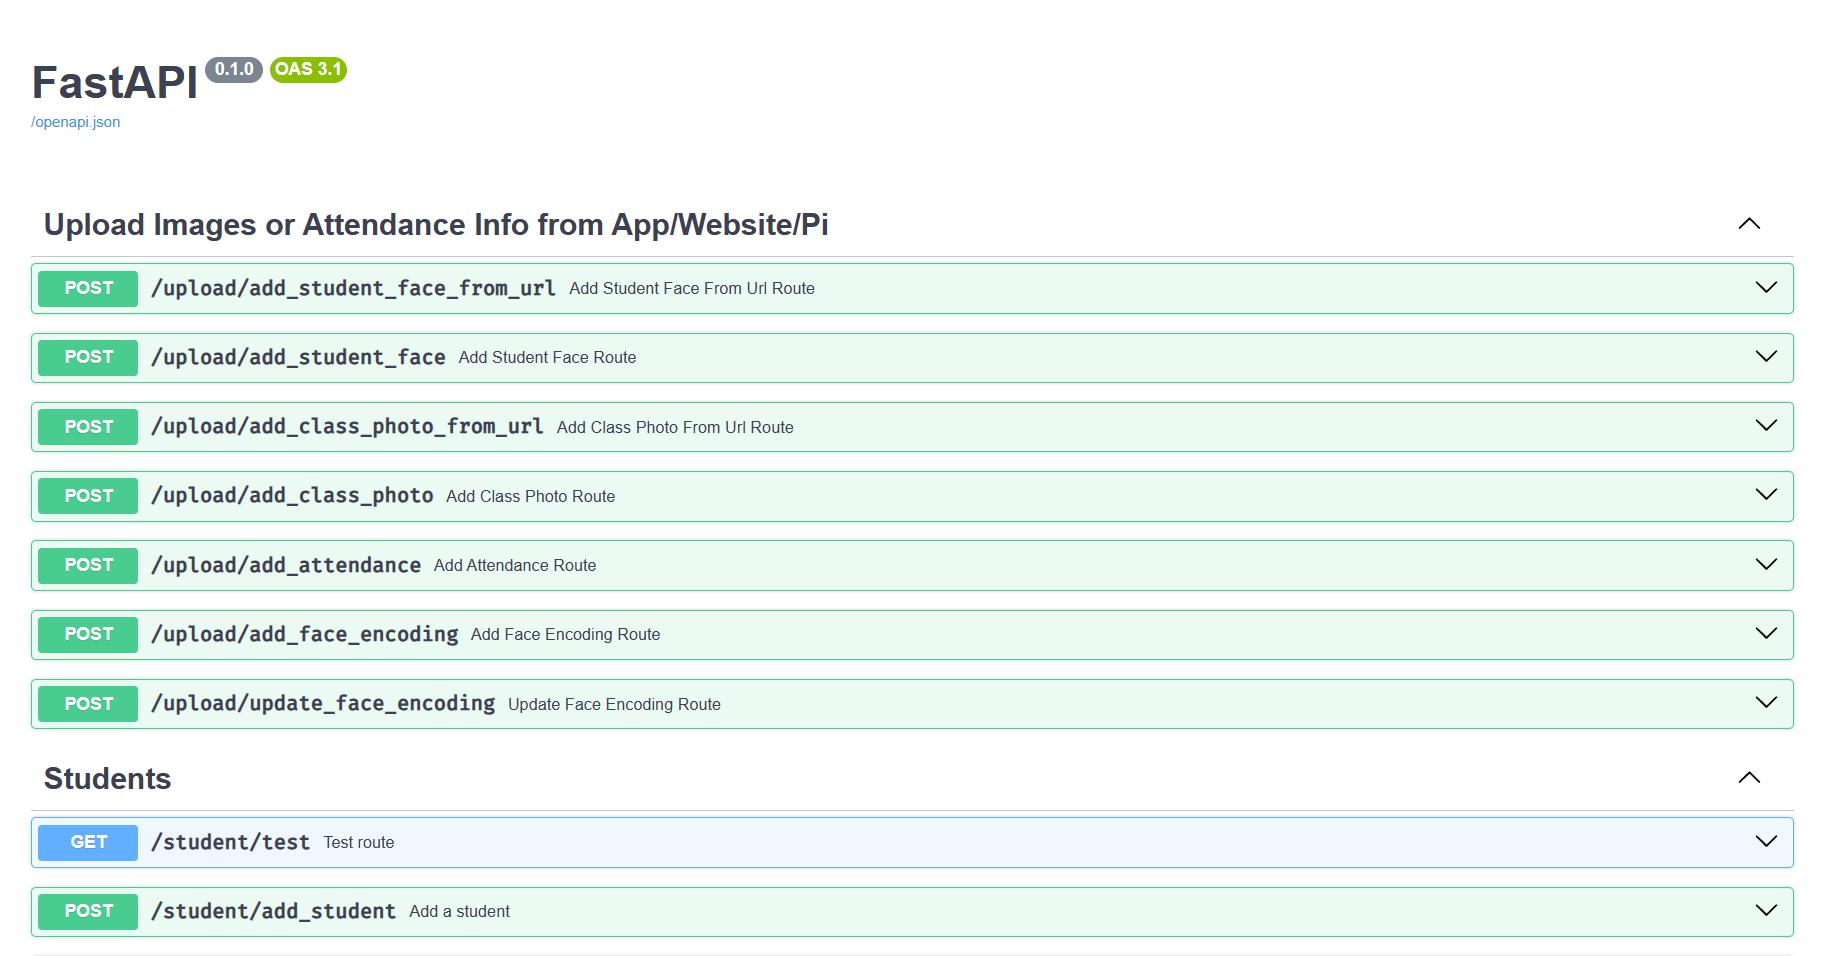
\includegraphics[width=0.95\textwidth]{../imgs/swagger 1.jpg}
    \caption{Swagger UI for API documentation (Krishnaraj Thadesar’s contribution).}
    \label{fig:swagger_ui}
\end{figure}
\begin{figure}[H]
    \centering
    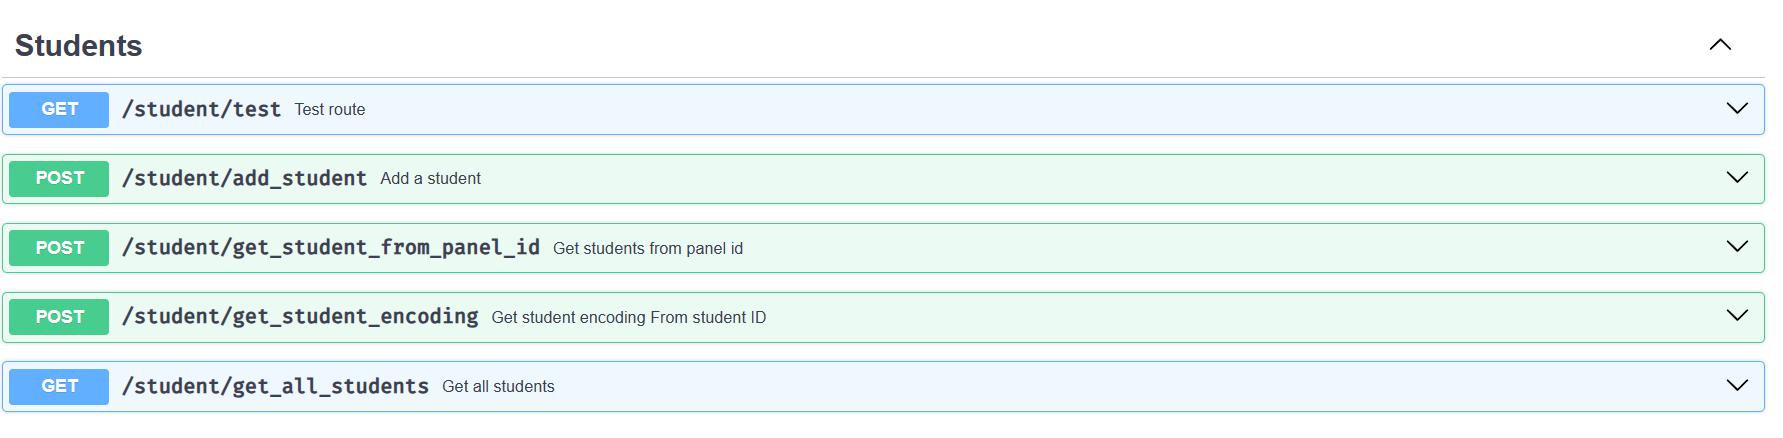
\includegraphics[width=0.95\textwidth]{../imgs/swagger 2.jpg}
    \caption{Swagger UI for API documentation (Krishnaraj Thadesar’s contribution).}
    \label{fig:swagger_ui}
\end{figure}
\begin{figure}[H]
    \centering
    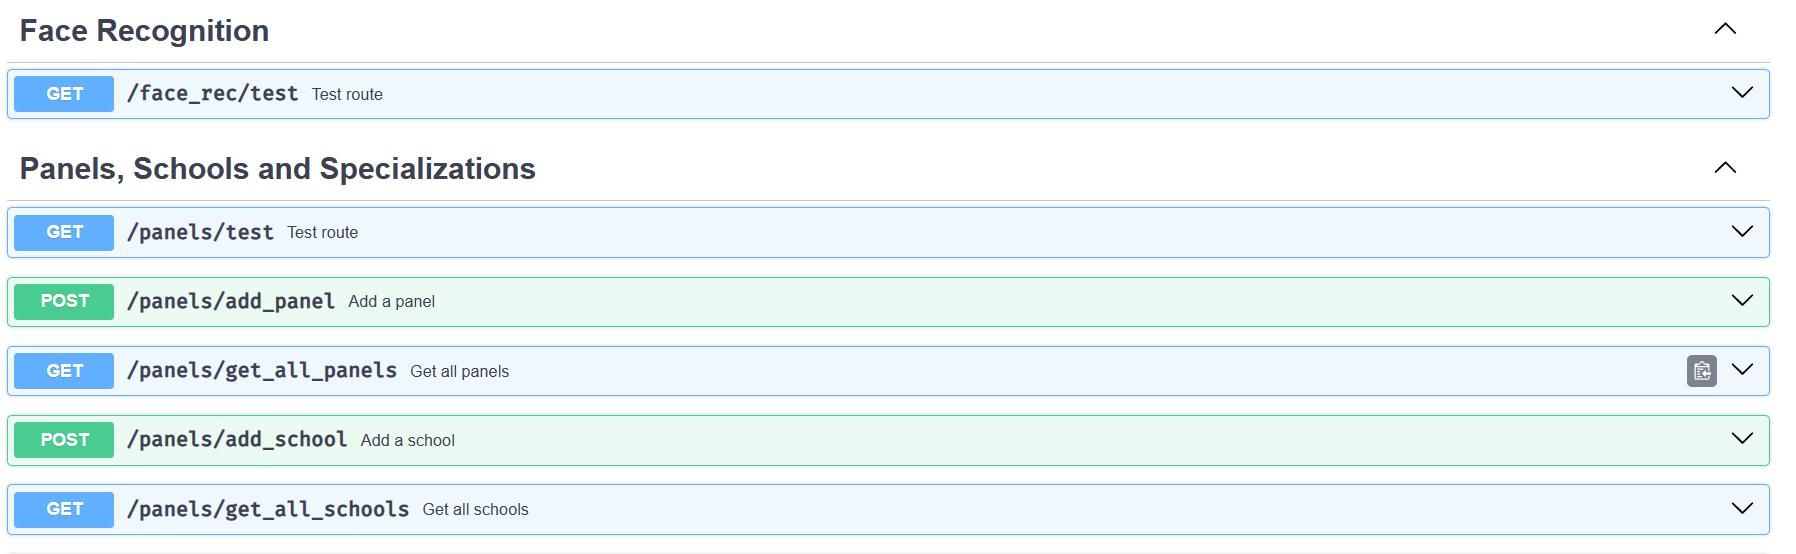
\includegraphics[width=0.95\textwidth]{../imgs/swagger 3.jpg}
    \caption{Swagger UI for API documentation (Krishnaraj Thadesar’s contribution).}
    \label{fig:swagger_ui}
\end{figure}
\subsection*{Module Interfaces}
The FastAPI application exposes the following routes (defined in \texttt{main.py} and router files):

\begin{itemize}
  \item \textbf{Add Attendance}  
    \texttt{POST /api/v1/add\_attendance}  
    \textit{Request body:}
    \begin{verbatim}
{
  "room_id": "Room ID",
  "subject_id": "Subject ID",
  "teacher_id": "Teacher ID",
  "panel_id": "Panel ID",
  "start_time": "10:00",
  "end_time": "11:00"
}
    \end{verbatim}

  \item \textbf{Add Image}  
    \texttt{POST /api/v1/add\_image}  
    \textit{Request body:}
    \begin{verbatim}
{
  "room_id": "Room ID",
  "image": "Base64-encoded image"
}
    \end{verbatim}
    \textit{Response:}
    \begin{verbatim}
{
  "status": "success",
  "message": "Image added successfully"
}
    \end{verbatim}

  \item \textbf{Add Specialization}  
    \texttt{POST /api/v1/add\_specialization}

  \item \textbf{Add School}  
    \texttt{POST /api/v1/add\_school}

  \item \textbf{Add Panel}  
    \texttt{POST /api/v1/add\_panel}

  \item \textbf{Add Student}  
    \texttt{POST /api/v1/add\_student}

  \item \textbf{Add Face Image}  
    \texttt{POST /api/v1/add\_face\_image}

  \item \textbf{Add Face Encoding}  
    \texttt{POST /api/v1/add\_face\_encoding}

  \item \textbf{Add Teacher}  
    \texttt{POST /api/v1/add\_teacher}

  \item \textbf{Add Semester}  
    \texttt{POST /api/v1/add\_semester}

  \item \textbf{Add Subject}  
    \texttt{POST /api/v1/add\_subject}

  \item \textbf{Get Students}  
    \texttt{POST /api/v1/get\_students}

  \item \textbf{Get Teachers}  
    \texttt{POST /api/v1/get\_teachers}
\end{itemize}

\subsection*{Module Dependencies}
\begin{itemize}
  \item \texttt{face\_recognition} $\rightarrow$ \texttt{dlib}, \texttt{numpy}
  \item \texttt{FastAPI} $\rightarrow$ \texttt{uvicorn}, \texttt{pydantic}
  \item MongoDB driver (\texttt{motor})
\end{itemize}

\subsection*{Module Design}
Layered architecture: Controller $\rightarrow$ Service $\rightarrow$ Model $\rightarrow$ Persistence; singleton face‐model loader; JWT authentication middleware.

\subsection*{Module Implementation}
\begin{itemize}
  \item Containerized services with Docker Compose.
  \item Approximately 1,200 lines of Python code.
  \item Integrated face\_recognition pipeline with error handling.
\end{itemize}

\subsection*{Module Testing Strategies}
\begin{itemize}
  \item Unit tests via \texttt{pytest} (coverage >= 85\%).
  \item Mocked face detection for CI.
  \item Postman end‐to‐end smoke tests.
\end{itemize}

\subsection*{Module Deployment}
\begin{itemize}
  \item Fully hosted on local Docker Compose setup.
  \item Single‐command bring‐up of all services (backend, database, model).
  \item Manual rollback by re‐deploying previous Docker image versions.
\end{itemize}

\chapter{Individual Contribution}

\section{Problem Statement}
Support the full-stack development cycle by contributing to UI design, API development, research, testing, and deployment for the Attendance-Assistant system.

\section{Student Details}
\textbf{Parth Zarekar} \\
\textbf{PRN:} 1032210846 \\
\textbf{Roll Number:} 09 \\
\textbf{Panel:} A \\

\section{Module Title}
Full-Stack Support \& Research


\section{Project Module Scope}
Assisted across UI design, backend API development, model-training research, paper drafting, testing, and deployment.
\begin{figure}[H]
    \centering
    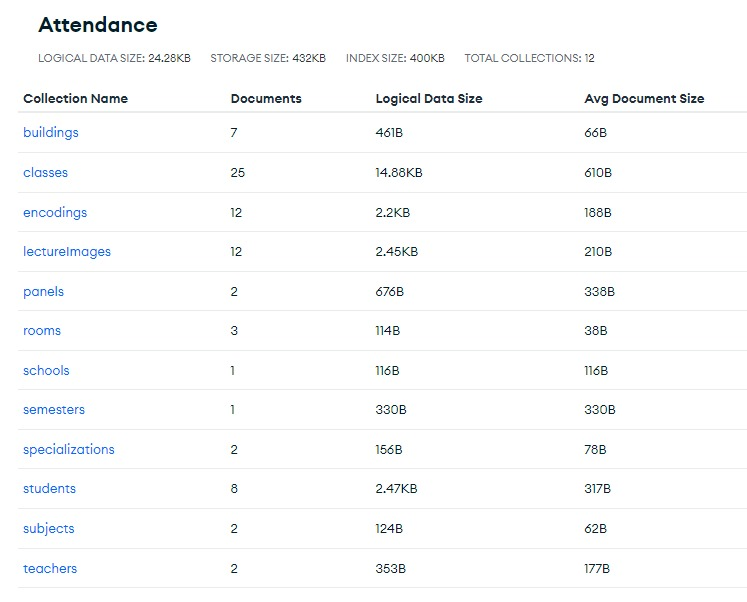
\includegraphics[width=0.8\textwidth]{../imgs/mongo.jpg}
    \caption{MongoDB Collections (Parth Zarekar’s area)}
    \label{fig:parth_mongodb}
\end{figure}

\begin{figure}[H]
    \centering
    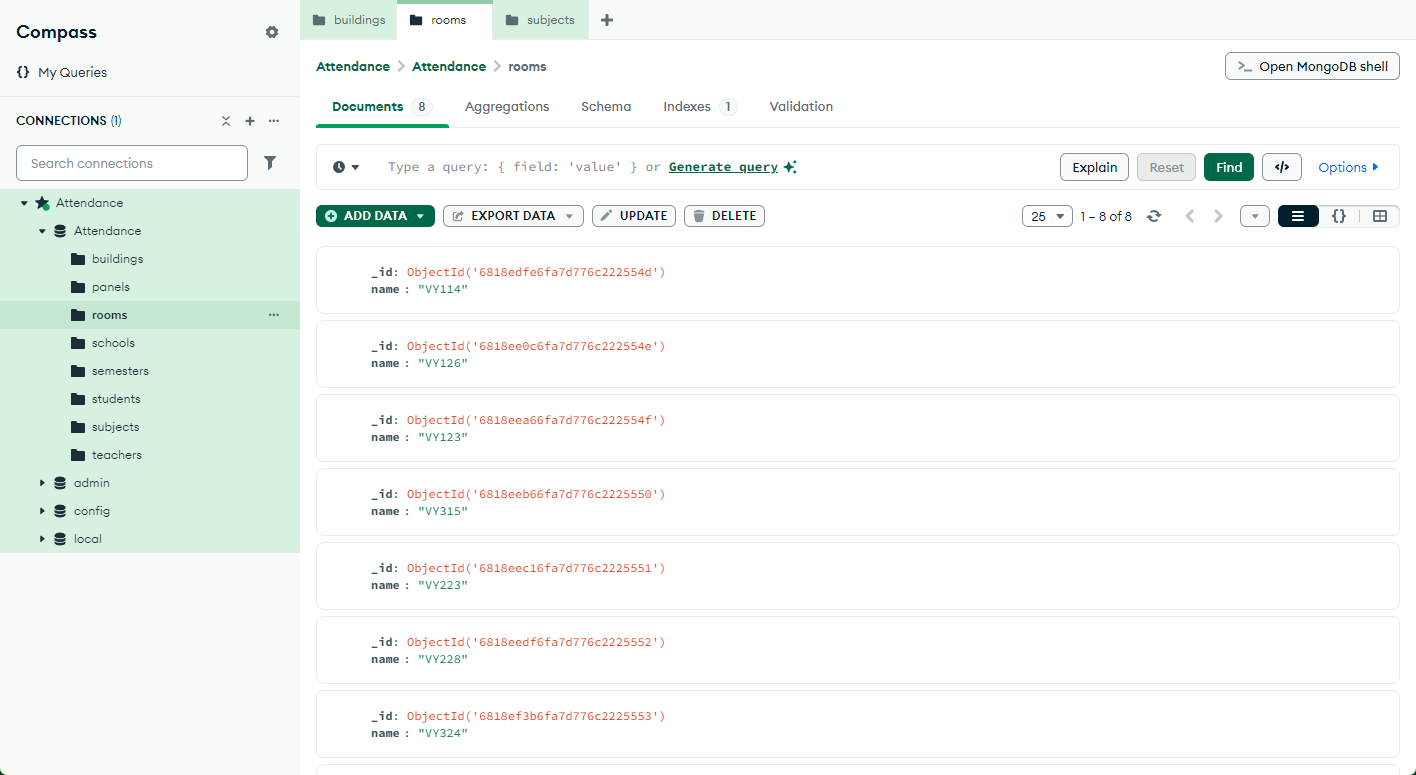
\includegraphics[width=0.8\textwidth]{../imgs/Mongo 1.png}
    \caption{MongoDB Collections (Parth Zarekar’s area)}
    \label{fig:parth_mongodb}
\end{figure}
\begin{figure}[H]
    \centering
    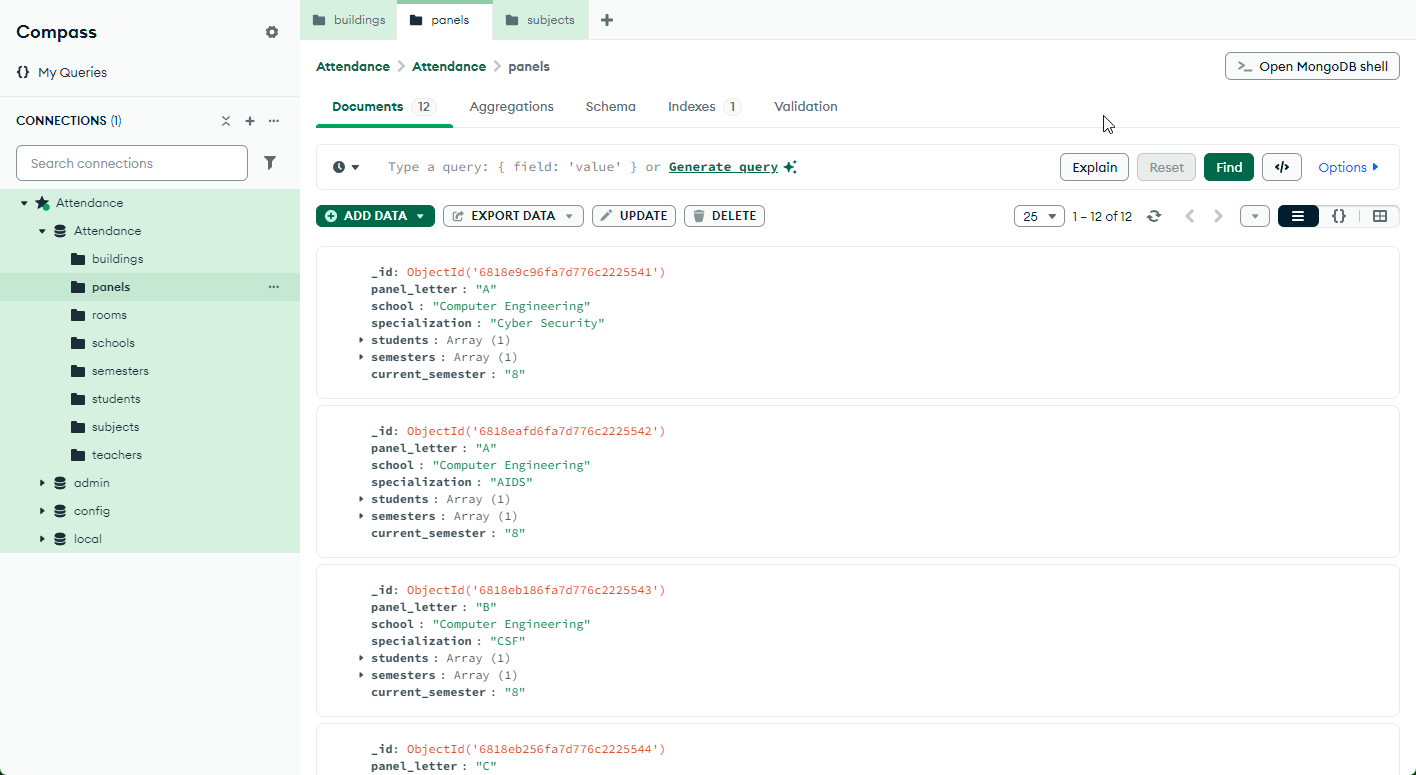
\includegraphics[width=0.8\textwidth]{../imgs/Mongo 2.png}
    \caption{MongoDB Collections (Parth Zarekar’s area)}
    \label{fig:parth_mongodb}
\end{figure}

\begin{figure}[H]
    \centering
    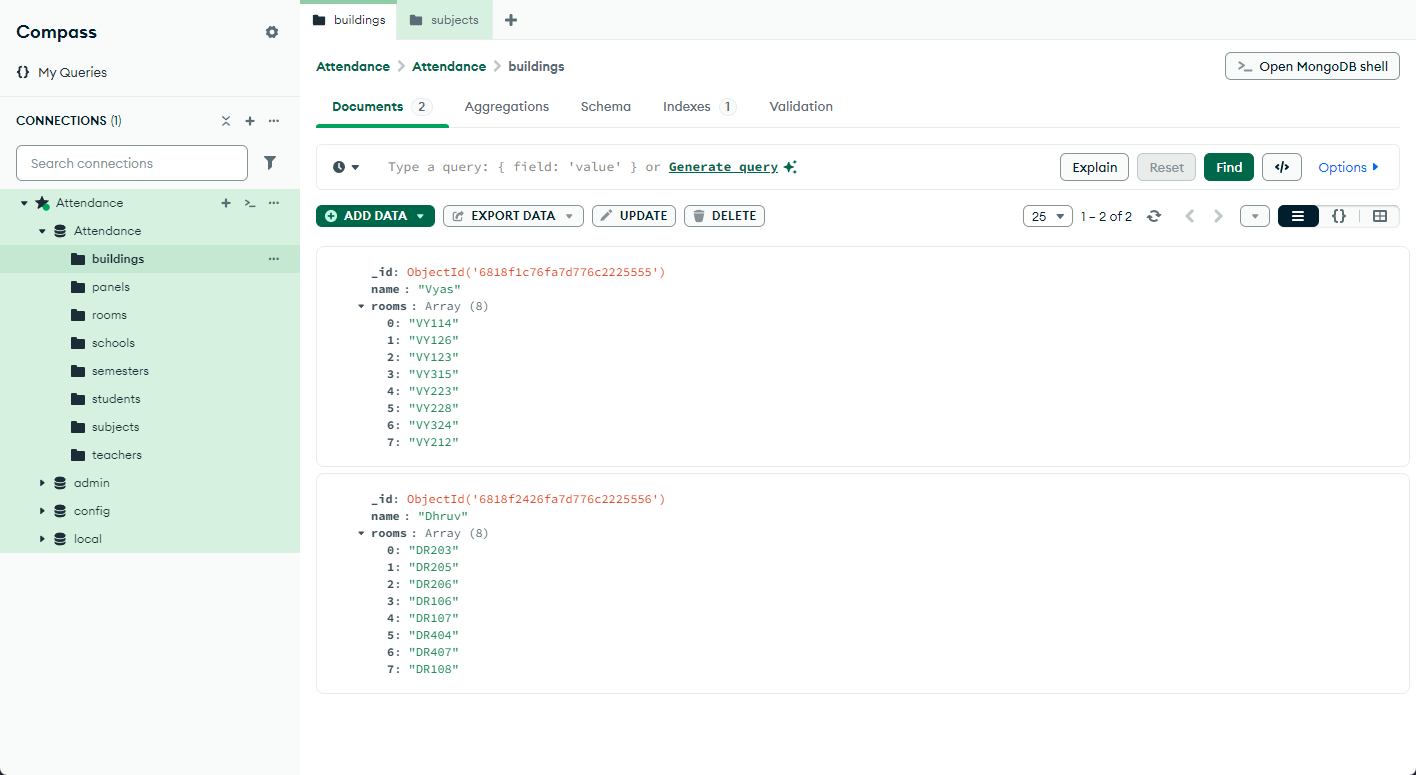
\includegraphics[width=0.8\textwidth]{../imgs/Mongo 3.png}
    \caption{MongoDB Collections (Parth Zarekar’s area)}
    \label{fig:parth_mongodb}
\end{figure}

\section{Project Modules – Individual Contribution}
\begin{enumerate}
  \item \textbf{Frontend:} Provided feedback and enhancements on Figma wireframes and UI flows.
  \item \textbf{Backend API:} Implemented core endpoints for image upload, face encoding, and attendance marking.
  \item \textbf{Model Research:} Supported training experiments and benchmark comparisons for face-recognition models.
  \item \textbf{Literature Research:} Drafted and edited sections of the project research paper on algorithm selection.
  \item \textbf{Testing:} Created and executed end-to-end tests (API smoke tests, basic UI checks).
  \item \textbf{Deployment:} Deployed Dockerized services to a basic AWS environment and configured DynamoDB storage.
\end{enumerate}
%----------------------------------------
\chapter{Individual Contribution}
%----------------------------------------
\section{Problem Statement}
Evaluate and benchmark multiple face-recognition algorithms; support model selection and integration.

\section{Student Details}
\textbf{Sourab Karad} \\
\textbf{PRN:} 1032211150 \\
\textbf{Roll Number:} 40 \\
\textbf{Panel:} A \\

\section{Module Title}
Algorithm Research \& Model Integration



\section{Project Module Scope}
Implementation and evaluation of face-recognition methods; performance reporting and API stub delivery.

\begin{figure}[H]
  \centering
  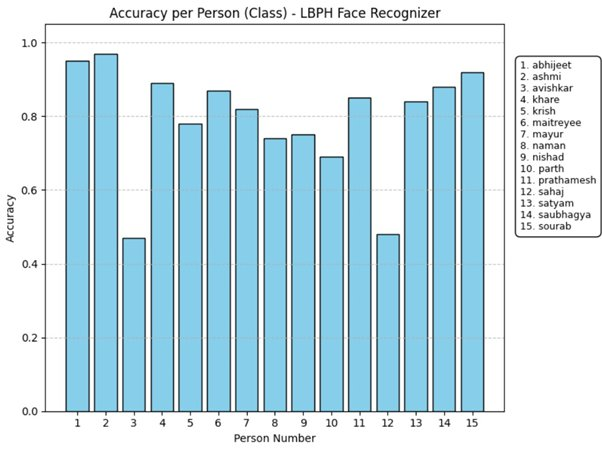
\includegraphics[width=.95\textwidth]{../imgs/model_1_per_person.jpg}
  \caption{Accuracy per Person (Class) - LBPH Face Recognizer}
\end{figure}


\begin{figure}[H]
  \centering
  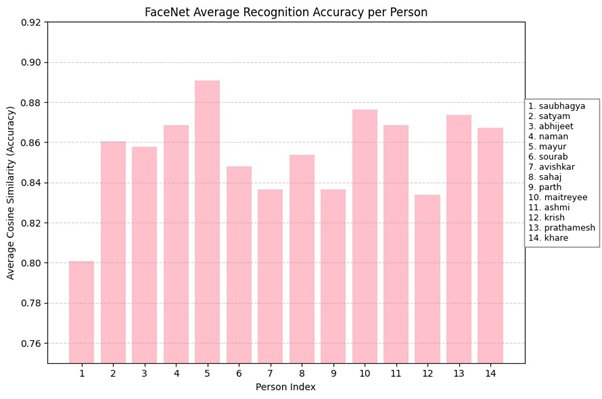
\includegraphics[width=.95\textwidth]{../imgs/model_2_per_person.jpg}
  \caption{Accuracy per Person (Class) - Facenet Face Recognizer}
\end{figure}


\begin{figure}[H]
  \centering
  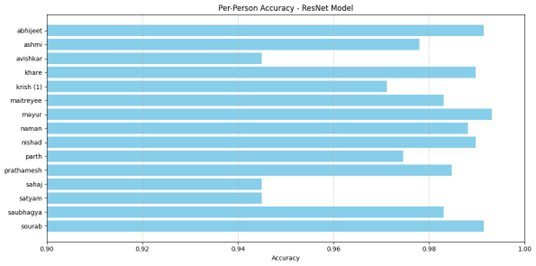
\includegraphics[width=.95\textwidth]{../imgs/model_3_per_person.jpg}
  \caption{Accuracy per Person (Class) - Resnet Face Recognizer}
\end{figure}

\begin{figure}[H]
    \centering
    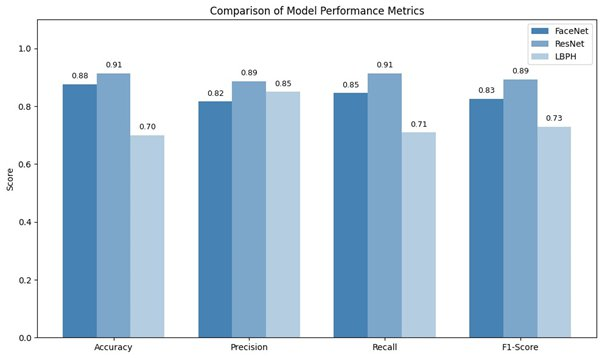
\includegraphics[width=0.8\textwidth]{../imgs/final_model_comp.jpg}
    \caption{Final Model Comparison (Sourab Karad’s results)} 
    \label{fig:sourab_graph}
\end{figure}
\section{Project Modules – Individual Contribution}
\begin{enumerate}
  \item \textbf{Hardware \& Software requirements:} GPU (RTX 2060), dlib, OpenCV, torch, scikit-learn, pandas.
  \item \textbf{Module Interfaces:} \texttt{train\_model.py}, \texttt{evaluate.py}; JSON output (\texttt{accuracy, precision, recall}).
  \item \textbf{Module Dependencies:} torch→torchvision; face\_recognition→dlib; numpy→pandas.
  \item \textbf{Module Design:} Abstract base classes; modular trainer \& evaluator.
  \item \textbf{Module Implementation:} ~800 LOC benchmarking harness; comparative plots in report.
  \item \textbf{Testing Strategies:} 5-fold cross-validation; confusion matrices.
  \item \textbf{Deployment:} Packaged ResNet model as pickle; provided Dockerfile snippet.
\end{enumerate}

%----------------------------------------
\chapter{Individual Contribution}
%----------------------------------------
\section{Problem Statement}
Design and build the cross-platform mobile app for attendance marking via facial capture.

\section{Student Details}
\textbf{Saubhagya Singh} \\
\textbf{PRN:} 1032211144 \\
\textbf{Roll Number:} 38 \\
\textbf{Panel:} A \\

\section{Module Title}
Flutter Front-End Application


\section{Project Module Scope}
Implement the Flutter-based UI for login, camera capture, attendance display, and offline support.
\begin{figure}[H]
    \centering
    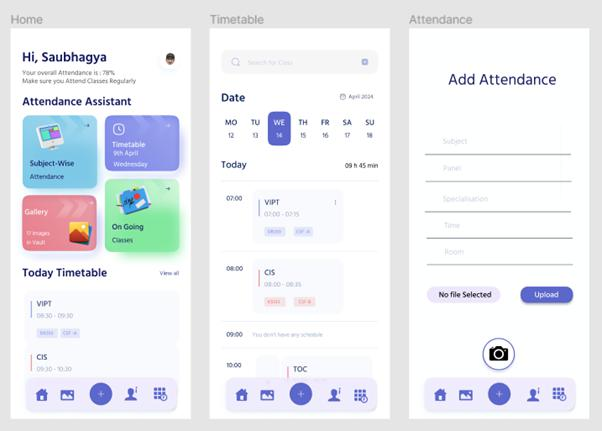
\includegraphics[width=0.95\textwidth]{../imgs/frontend.jpg}
    \caption{Frontend  (Saubhagya Singh’s contribution).}
    \label{fig:block_diagram_saubhagya}
\end{figure}

\section{Project Modules – Individual Contribution}
\begin{enumerate}
  \item \textbf{UI Design:} Assisted in Figma wireframes and refined user flows.
  \item \textbf{Flutter Development:} Built screens for login, camera preview, and attendance history.
  \item \textbf{Camera Integration:} Integrated device camera plugin and handled image capture.
  \item \textbf{Offline Support:} Added basic local caching to queue captures when offline.
  \item \textbf{Testing:} Performed manual UI tests on both Android and iOS emulators.
\end{enumerate}

\end{document}
